\documentclass{article}

\usepackage{amsmath,amssymb}
\usepackage{tikz}
\usepackage{pgfplots}
\usepackage{xcolor}
\usepackage[left=2.1cm,right=3.1cm,bottom=3cm,footskip=0.75cm,headsep=0.5cm]{geometry}
\usepackage{enumerate}
\usepackage{enumitem}
\usepackage{marvosym}
\usepackage{tabularx}
\usepackage[amsmath,thmmarks,standard]{ntheorem}
\usepackage{mathtools}

\usepackage[utf8]{inputenc}

\renewcommand*{\arraystretch}{1.4}
\newcommand{\E}{\mathbb{E}}

\newcolumntype{L}[1]{>{\raggedright\arraybackslash}p{#1}}
\newcolumntype{R}[1]{>{\raggedleft\arraybackslash}p{#1}}
\newcolumntype{C}[1]{>{\centering\let\newline\\\arraybackslash\hspace{0pt}}m{#1}}

\DeclareMathOperator{\tr}{tr}
\DeclareMathOperator{\Var}{Var}
\DeclareMathOperator{\Cov}{Cov}
\renewcommand{\E}{\mathbb{E}}

\newtheorem{thm}{Theorem}
\newtheorem{lem}{Lemma}

\title{\textbf{Einführung in die Logistik, Übung 1}}
\author{\textsc{Henry Haustein}}
\date{}

\begin{document}
	\maketitle
	
	\section*{Aufgabe 1}
	\begin{enumerate}[label=(\alph*)]
		\item grafische Darstellung von $\vec{G}$
		\begin{center}
			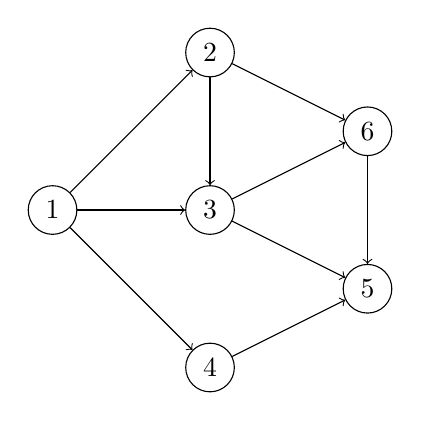
\begin{tikzpicture}
				\node[circle,draw=black, fill=white] (1) at (0,0) {1};
				\node[circle,draw=black, fill=white] (2) at (2,2) {2};
				\node[circle,draw=black, fill=white] (3) at (2,0) {3};
				\node[circle,draw=black, fill=white] (4) at (2,-2) {4};
				\node[circle,draw=black, fill=white] (5) at (4,-1) {5};
				\node[circle,draw=black, fill=white] (6) at (4,1) {6};
				
				\draw[->] (1) -- (2);
				\draw[->] (1) -- (3);
				\draw[->] (1) -- (4);
				\draw[->] (2) -- (3);
				\draw[->] (2) -- (6);
				\draw[->] (3) -- (6);
				\draw[->] (3) -- (5);
				\draw[->] (4) -- (5);
				\draw[->] (6) -- (5);
			\end{tikzpicture}
		\end{center}
		\item Die Adjazenzmatrix $A$ lautet:
		\begin{align}
			A(G) = \begin{array}{c|cccccc}
				& 1 & 2 & 3 & 4 & 5 & 6 \\
				\hline
				1 & 0 & 0 & 0 & 0 & 0 & 0 \\
				2 & 1 & 0 & 0 & 0 & 0 & 0 \\
				3 & 1 & 1 & 0 & 0 & 0 & 0 \\
				4 & 1 & 0 & 0 & 0 & 0 & 0 \\
				5 & 0 & 0 & 1 & 1 & 0 & 1 \\
				6 & 0 & 1 & 1 & 0 & 0 & 0 \\
			\end{array} \notag
		\end{align}
		Die Ausgangsgrade sind die Spaltensummen, die Eingangsgrade die Zeilensummen
		\item Zyklenfreiheit ist gegeben, für topologische Sortierung müssen die Knoten 5 und 6 zu 6 und 5 umnummeriert werden.\footnote{Ein Graph ist dann topologisch sortiert, wenn die Adjazenzmatrix eine echte untere Dreiecksmatrix ist, das heißt auch auf der Hauptdiagonalen stehen nur noch Nullen.}
		\item zugehörige Graph $G$
		\begin{center}
			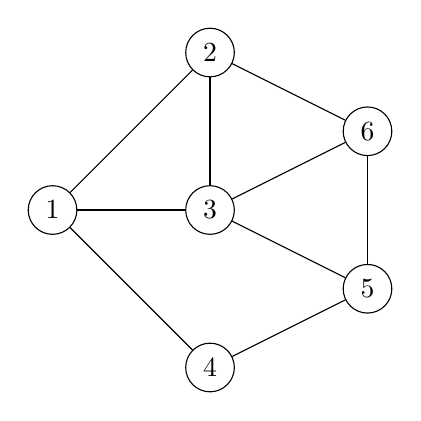
\begin{tikzpicture}
				\node[circle,draw=black, fill=white] (1) at (0,0) {1};
				\node[circle,draw=black, fill=white] (2) at (2,2) {2};
				\node[circle,draw=black, fill=white] (3) at (2,0) {3};
				\node[circle,draw=black, fill=white] (4) at (2,-2) {4};
				\node[circle,draw=black, fill=white] (5) at (4,-1) {5};
				\node[circle,draw=black, fill=white] (6) at (4,1) {6};
				
				\draw (1) -- (2);
				\draw (1) -- (3);
				\draw (1) -- (4);
				\draw (2) -- (3);
				\draw (2) -- (6);
				\draw (3) -- (6);
				\draw (3) -- (5);
				\draw (4) -- (5);
				\draw (6) -- (5);
			\end{tikzpicture}
		\end{center}
		$\vec{G}$ ist offensichtlich nicht stark zusammenhängend, da z.B. $1\not\leftrightsquigarrow 2$ gilt. Aber da $G$ zusammenhängend ist, ist $\vec{G}$ wenigstens schwach zusammenhängend.
	\end{enumerate}

	\section*{Aufgabe 2}
	\begin{enumerate}[label=(\alph*)]
		\item Die Graphen $\vec{G}$ und $G=Z(\vec{G})$
		\begin{center}
			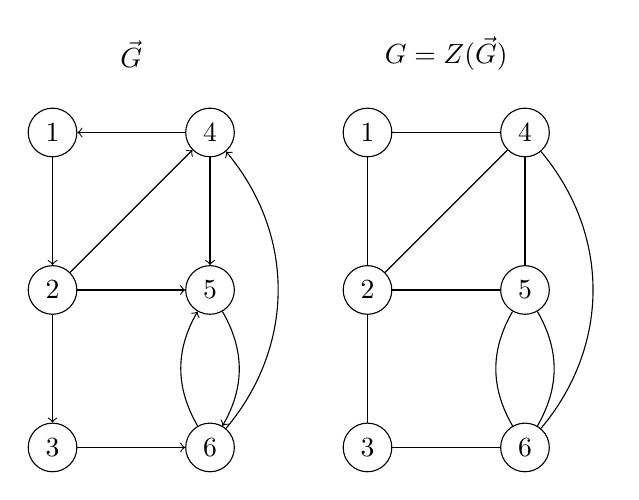
\begin{tikzpicture}
				\node[circle,draw=black, fill=white] (1) at (0,0) {1};
				\node[circle,draw=black, fill=white] (2) at (0,-2) {2};
				\node[circle,draw=black, fill=white] (3) at (0,-4) {3};
				\node[circle,draw=black, fill=white] (4) at (2,0) {4};
				\node[circle,draw=black, fill=white] (5) at (2,-2) {5};
				\node[circle,draw=black, fill=white] (6) at (2,-4) {6};
				
				\draw[->] (1) -- (2);
				\draw[->] (2) -- (3);
				\draw[->] (3) -- (6);
				\draw[->] (2) -- (5);
				\draw[->] (4) -- (1);
				\draw[->] (2) -- (4);
				\draw[->] (4) -- (5);
				\draw[->] (5) to[bend left=30] (6);
				\draw[->] (6) to[bend right=40] (4);
				\draw[->] (6) to[bend left=30] (5);
				
				\node at (1,1) {$\vec{G}$};
				\node at (5,1) {$G=Z(\vec{G})$};
				
				\node[circle,draw=black, fill=white] (a1) at (4,0) {1};
				\node[circle,draw=black, fill=white] (a2) at (4,-2) {2};
				\node[circle,draw=black, fill=white] (a3) at (4,-4) {3};
				\node[circle,draw=black, fill=white] (a4) at (6,0) {4};
				\node[circle,draw=black, fill=white] (a5) at (6,-2) {5};
				\node[circle,draw=black, fill=white] (a6) at (6,-4) {6};
				
				\draw (a1) -- (a2);
				\draw (a2) -- (a3);
				\draw (a3) -- (a6);
				\draw (a2) -- (a5);
				\draw (a4) -- (a1);
				\draw (a2) -- (a4);
				\draw (a4) -- (a5);
				\draw (a5) to[bend left=30] (a6);
				\draw (a6) to[bend right=40] (a4);
				\draw (a6) to[bend left=30] (a5);
			\end{tikzpicture}
		\end{center}
		\item Es gilt $A(Z(\vec{G})) = A(\vec{G}) + A(\vec{G})^T$
		\begin{align}
			A(\vec{G}) &= \begin{array}{c|cccccc}
				& 1 & 2 & 3 & 4 & 5 & 6 \\
				\hline
				1 & 0 & 0 & 0 & 1 & 0 & 0 \\
				2 & 1 & 0 & 0 & 0 & 0 & 0 \\
				3 & 0 & 1 & 0 & 0 & 0 & 0 \\
				4 & 0 & 1 & 0 & 0 & 0 & 1 \\
				5 & 0 & 1 & 0 & 1 & 0 & 1 \\
				6 & 0 & 0 & 1 & 0 & 1 & 0
			\end{array} \notag \\
			A(Z(\vec{G})) &= \begin{array}{c|cccccc}
				& 1 & 2 & 3 & 4 & 5 & 6 \\
				\hline
				1 & 0 & 1 & 0 & 1 & 0 & 0 \\
				2 & 1 & 0 & 1 & 1 & 1 & 0 \\
				3 & 0 & 1 & 0 & 0 & 0 & 1 \\
				4 & 1 & 1 & 0 & 0 & 1 & 1 \\
				5 & 0 & 1 & 0 & 1 & 0 & 1 \\
				6 & 0 & 0 & 1 & 1 & 1 & 0
			\end{array} \notag
		\end{align}
		\item Graph $\vec{G}$:
		\begin{itemize}
			\item offene Hamiltonsche Linie: (4,1,2,3,6,5)
			\item keine Eulersche Linie möglich, da Knoten 5 nicht 3 mal besucht, aber nur einmal verlassen werden kann
		\end{itemize}
		Graph $G$
		\begin{itemize}
			\item geschlossene Hamiltonsche Linie: [1,2,3,6,5,4,1]
			\item offene Eulersche Linie: [6,5,2,3,6,4,1,2,4,5]
		\end{itemize}
	\end{enumerate}
	
	\section*{Aufgabe 3}
	\begin{enumerate}[label=(\alph*)]
		\item Wir zeichnen den Graphen zuerst
		\begin{center}
			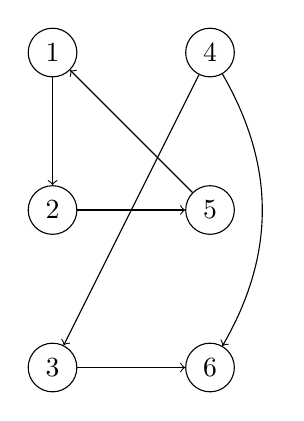
\begin{tikzpicture}
				\node[circle,draw=black, fill=white] (1) at (0,0) {1};
				\node[circle,draw=black, fill=white] (2) at (0,-2) {2};
				\node[circle,draw=black, fill=white] (3) at (0,-4) {3};
				\node[circle,draw=black, fill=white] (4) at (2,0) {4};
				\node[circle,draw=black, fill=white] (5) at (2,-2) {5};
				\node[circle,draw=black, fill=white] (6) at (2,-4) {6};
				
				\draw[->] (1) -- (2);
				\draw[->] (2) -- (5);
				\draw[->] (5) -- (1);
				\draw[->] (3) -- (6);
				\draw[->] (4) to[bend left=30] (6);
				\draw[->] (4) -- (3);
			\end{tikzpicture}
		\end{center}
		\begin{align}
			A(\vec{G}) &= \begin{array}{c|cccccc}
				& 1 & 2 & 3 & 4 & 5 & 6 \\
				\hline
				1 & 0 & 0 & 0 & 0 & 1 & 0 \\
				2 & 1 & 0 & 0 & 0 & 0 & 0 \\
				3 & 0 & 0 & 0 & 1 & 0 & 0 \\
				4 & 0 & 0 & 0 & 0 & 0 & 0 \\
				5 & 0 & 1 & 0 & 0 & 0 & 0 \\
				6 & 0 & 0 & 1 & 1 & 0 & 0
			\end{array} \notag
		\end{align}
		Man kann den Graphen in 2 Untergraphen unterteilen, das heißt $\vec{G}$ ist nicht zusammenhängend.
	\end{enumerate}
	
\end{document}